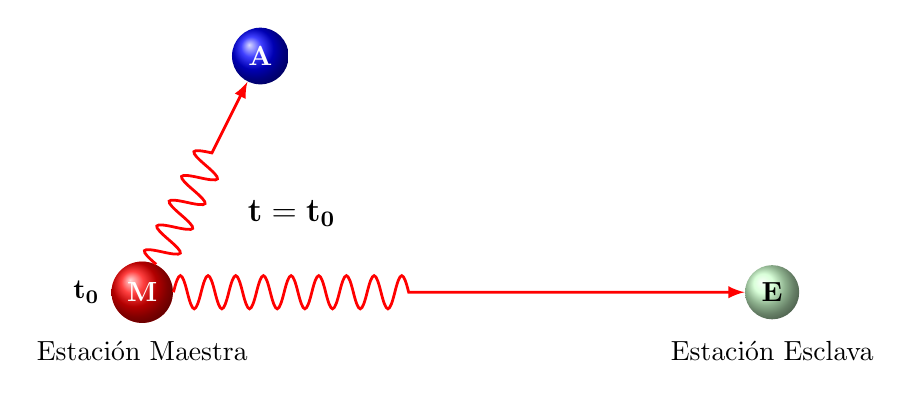
\begin{tikzpicture}[scale=1]
\usetikzlibrary{snakes}
\usetikzlibrary{calc}

%  \draw[help lines, green!70, step=0.5] (0,0) grid (9,4);
	% Impulso tiempo t0

	\node[circle, 
				shading=ball, 
				fill=red!50, 
				ball color=red,
				text=white
				] (M) at (0,0) {$\bf M$};

	\node[circle,
				shading=ball, 
				ball color=green!20,
%				text=white
				] (E) at (8,0) {$\bf E$};

	\node[circle,
				shading=ball,
%				ball color=black,
				text=white
				] (A) at (1.5,3) {$\bf A$};

	\draw (M) ++(0.0,-0.5) node[anchor=north] {Estaci\'on Maestra}; 
	\draw (E) ++(0.0,-0.5) node[anchor=north] {Estaci\'on Esclava}; 
%	\draw[-latex, line width=1] (F2) -- (P1); 
%	\draw[-latex, line width=1] (F1) -- (F2); 

%	\draw[anchor=west] at (F1) {$t_0$};
	\draw  (M) ++(-1.0,0) node[anchor=west] {$\bf t_0$} ;
	\draw  (M) ++( 1.9,1.0) node {\large $\bf t = t_0$} ;

	\draw[-latex, line width=1, 
				snake=coil, 
				segment aspect=0, red, 
				line after snake=1cm,
				segment amplitude=6pt
				] 	(M) -- (A);
%				$($(F1)!0.40cm!(P1)$) -- ($(F1)!1.5cm!(P1)$); 

	\draw[-latex, line width=1, 
				snake=coil, 
				segment aspect=0, red, 
				line after snake=4cm,
				segment amplitude=6pt
				] (M) -- (E); 



\end{tikzpicture}